\section{OpenGL aplikacijsko sučelje}

OpenGL razvio se kao nasljednik IrisGL-a \footnote{engl. Integrated Raster Imaging System Graphics Library}. Njegova glavni nedostatak bio je što su mogućnosti samog sučelja ovisile o mogućnostima sklopovlja, te se nije mogao primijeniti na različitim uređajima. Zbog potrebe za iyradom standarda, početkom 1990-tih godina tvrtka Silicon Graphics Inc. (SCI) započela je sa izradom OpenGL specifikacije kako bi formalno definirala aplikacijsko programsko sučelje (API) prema grafičkim karticama. Godine 1992., prva verzija OpenGl-a je objavljena. Od 2016.g. ne-profitna grupa Khronos zadužena je za razvoj OpenGL-a \cite{opengl-wiki-hostory}.

Primarni zadatak ovog API-a je prikaz 2D i 3D vektorske grafike. On omogućuje komunikaciju sa grafičkim procesorom (GPU) s ciljem sklopovskog ubrzanja grafičkog prikaza, neovisno o programskom jeziku i operativnom sustavu.

Zbog svoje proširenosti i upotrebe, postao je industrijski standard. Podržan je na velikom broju uređaja,od računala do pametnih telefona. Ima široku primjenu u industriji (CAD \footnote{engl. Computer-Aided Design}, GIS \footnote{engl. Geographic Information System}, simulacijama i vizualizacijama) te u izradi računalnih igara.

\subsection{OpenGL grafički cjevovod}

U svojim početcima, prilikom rada s računalnom grafikom nije bilo puno mjesta za manipulaciju sa slikom. Grafičko sklopovlje nije omogućavalo puno manipulacije sa bojom i pozicijom objekata na ekranu. Računalo je \emph{slalo} opise vektore i teksturu koju oni stvaraju, dok su grafičke kartice bila zadužene za stvaranje slike iz ta dva dobivena podatka.

Takav način rada podrazumijevao je da se sva potreban kalkulacija (tranformacija koordinata - pomak) i sjenčanje prethodno odrade na samom računalu, prije nego što se pošalju grafičkoj kartici za prikaz. Glavni nedostatak tog pristupa je što svu kalkulaciju morala obrađivati centralna procesorska jedinica (CPU) koja osim što nije bila dizajnirana za takve operacije, je morala obrađivati i niz drugih podataka istovremeno.

Iz tog razloga, pojavila se potreba za programabilnim \emph{grafičkim cjevovodom} \footnote{engl. Graphival pipline} koji bi omogućio manipulaciju podacima na grafičkoj kartici. OpenGL cjevovod sastoji se od 7. komponenti\cite{opengl-wiki-pipeline}, prikazanih na Slici \ref{fig:pipeline}.

\begin{figure}[H]
\caption{Dijagram toka OpenGL cjevovoda}
\label{fig:pipeline}
\begin{center}
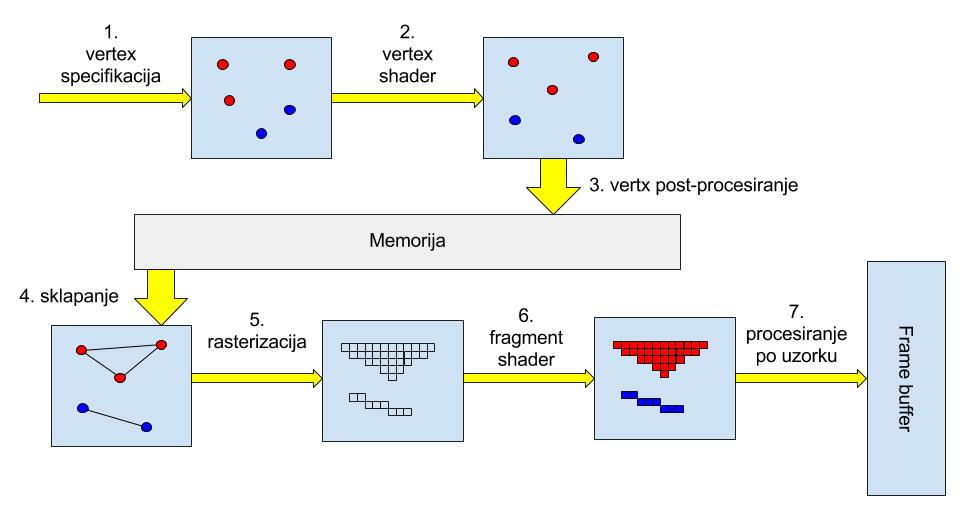
\includegraphics[scale=0.3]{pipeline.jpg}
\end{center}
\end{figure}

\begin{enumerate}
\item \textbf{Vertex specifikacija:} U ovom koraku aplikacija prenosi podatke grafičkoj kartici - opise vertex-a \footnote{Točka u trodimenzionalnom prostoru. Osim pozicije, vertex može sadržavati i druge informacije, poput boje}. Način na koji će se vertex tumačiti/iscrtavati se kasnije obrađuje.

\item \textbf{Vertex shader:} Izvršavanje vertex shader korisničkog programa. Cilj ovog koraka je transformirati ulaznu poziciju vektora u njegov krajnji oblik. Ovdje se najčešće vrše transformacije s ciljem postizanja pogleda iz perspektive, rotacije i uvećanja. U ovoj fazi pokreće se i geometrijski shader, koji radi kao i vertex shader, samo na razini ploha.

\item \textbf{Vertx post-procesiranje:} Rezultati prošlog koraka spremaju se za na to predviđene memorijske lokacije.

\item \textbf{Sklapanje ploha:} U ovome koraku, grafički procesor sklapa ploha od unaprijed obrađenih vertexa.

\item \textbf{Rasterizacija:} Sklopljene plohe razdvajaju se na fragment koji se prosljeđuju dalje kako bi im se odredila boja, odnosno tekstura.

\item \textbf{Fragment shader:} Svaki fragment se prosljeđuje korisničkom programu fragment shaderu) čiji izlaz predstavlja boju danoga fragmenta.

\item \textbf{Procesiranje po uzorku:} Ovaj korak služi za izvršavanje raznih testova koji mogu utjecati na krajnji rezultat, primjerice test dubine (U koliko se fragment nalazi iza nekog drugog, vjerojatno neće biti prikazan). Također ovdje se vrše operacije i odbacivanja fragmenata koji nisu na vidljivom djelu ekrana, stapanje boja i sl.

\end{enumerate}

Kod ovoga koraka bitno je napomenuti kako su procesi optimizirani na način da se što više operacija može izvršavati paralelno. Današnje grafičke kartice imaju i po nekoliko stotina jezgri koje mogu paralelno raditi, što omogućava paralelno izvršavanje nekoliko shadera istovremeno, što u konačnici rezultira velikom brzinom obrade podataka, nešto što nije moguće na centralnoj procesorskoj jedinici,

\subsection{Shaderi i GLSL}

Kao što je opisano u prethodnom poglavlju, shaderi su najbitnije komponente progamabilnog grafičkog cjevovoda. Oni su zapravo male korisničke aplikacije koje se izvode paralelno, i obrađuju manji set informacija od jednom.

Korisničke aplikacije za vertex i fragment shader (opcinoalno i geometrijski) se dostavljaju grafičkoj kartici, i zatim komapjliraju u jedan \emph{program} koji se izvodi u sklopu cjevovoda. Bitno je napomenuti da je moguće prirediti više od jednog programa, te ih mijenjati tokom izvođenja.

Shaderi se pišu programskom jeziku koji je posebno dizajniran za ovu primjenu - GLSL \footnote{engl. OpenGL Shading Language}. GLSL programski jezik baziran je na C programskom jezu, i dio je OpenGL specifikacije. Razlikuje se od C-a u nekoliko ključnih stvari: Nadograđen je da podržava matrične operacije i tipove podataka. Za razliku od C-a, ne podržava preopterećenje funkcija na osnovu ulaznih parametara niti rekurzivne funkcije.

\subsection{Transformacije objekta}

Kako je ranije spomenuto, ideja programabilnog grafičkog cjevovoda je pomaknuti grafičke kalkulacije sa centralnog procesora na grafički procesor. To prvenstveno znači rekalkulaciju pozicije i oblika objekta uslijed pomaka samog objekta ili kamere. To se najčešće vrši množenjem kordinata pojedine točke objekta sa takozvanom MVP \footnote{engl. Model View Projection} matricom. MVP matrica se sastoji iz tri dijela \cite{opengl-es-mvp}:

\begin{enumerate}
\item \textbf{Matrica modela:} Matrica koja opisuje osnovne transformacije modela: translaciju, rotaciju i skaliranje. Dobiva se množenjem istoimenih matrica.

\item \textbf{Matrica scene (view):} Budući da se u računalnoj grafici kamera ne pomiče, već se pomiče svijet oko nje - ova matrica služi kako bi ispravno pozicionirala objekt u odnosu na kameru.

\item \textbf{Projekcijska matrica:} Služi za definiranje transformacije s ciljem postizanja željene projekcije. To je najčešće perspektivna projekcija, no može biti ortogonalna i bilo kako drugo definirana.
\end{enumerate}

Sam izračun MVP matrice, obično se vršri na centralnoj procesorskoj jedinici i kao takav se dostavlja grafičkoj kartici. Ona je zatim zadužena da svaki pojedini vertex pozicionira na pravo mjesto, uzimajući MVP matricu u obzir - pomnoži koordinate vertxa sa MVP matricom da dobije konačnu poziciju u prostoru.

Na ovaj način, smanjuje se količina posla koju obavlja centralna procesorska jedinica. Ona samo računa način tranformacije, dok se stvarni pomak modela odvija na samoj grafičkoj kartici, koja je u mogućnosti to obaviti neusporedivo brže, za svaki vertex posebno.

\subsection{WebGL}

Ukratko u tome što je WebGL i kako se raylikuje od ostalih OpenGL implementacija

\subsection{Modeli u Three.js JSON formatu}

Struktura formata